\section{Experiment with Pozyx}
We have created an experiment to test how accurate the tags in Pozyx are.
The primary goal of the experiment was to test the accuracy, but a biproduct of the experiment was to see how many update frequencies there were with each tag.

\subsection{Setup}
The current settings goes for best precision, but gives a smaller amount of updates.
% Uddyb hvilke settings det er.
The setup of the experiment as seen on \autoref{fig:experiment-setup}. 
The experiment was conducted indoors in Novi 9. 
\texttt{0x632b} and \texttt{0x676e} was mounted on a wall 240 centimeters apart.
\texttt{0x6738} and \texttt{0x676c} was mounted on a bulletin board.
There was chosen different heights as Pozyx documentation suggests that not all anchors should have the same height.
%uddyb

\begin{figure}[H]
    \centering
    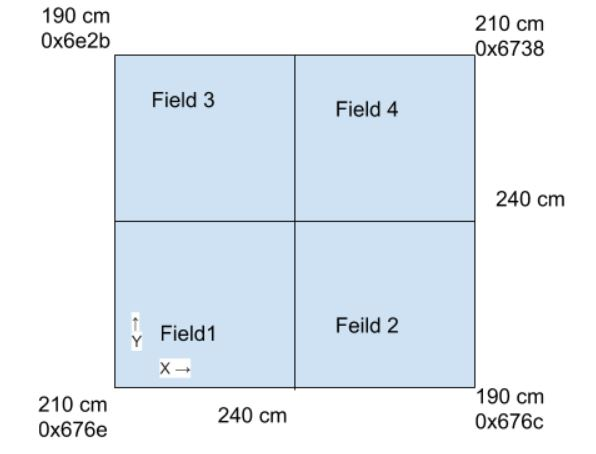
\includegraphics[width=0.6\linewidth]{experiment-setup.JPG}
    \caption{The setup of the experiment with the anchors and the height in the corners.}
    \label{fig:experiment-setup}
\end{figure}
\noindent
The fields was a blackboard where lines were drawn for each 10 centimeters to know the actual position as seen on.

\begin{figure}[H]
    \centering
    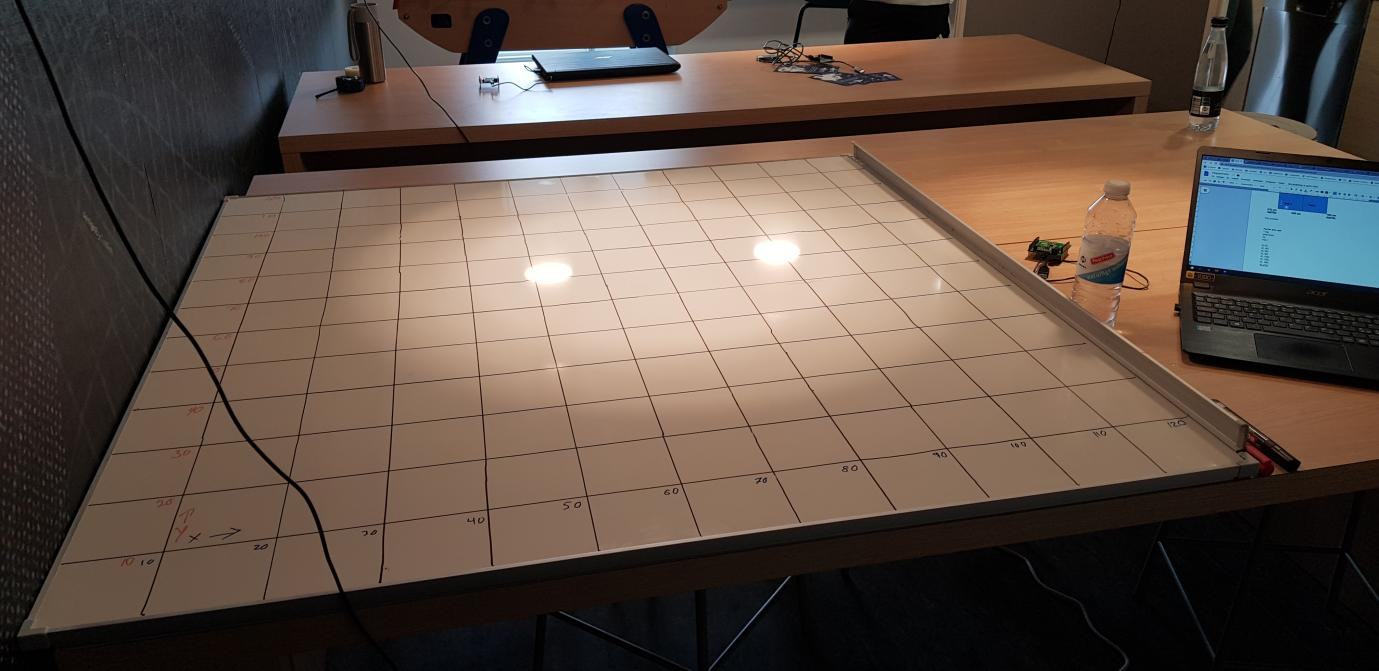
\includegraphics[width=0.8\linewidth]{experiment-blackboard.png}
    \caption{The blackboard with the drawn positions.}
    \label{fig:experiment-blackboard}
\end{figure}
 
\subsection{Precision with 1 tag}
As can be seen on \autoref{Tab:one-tag-experiment-result}

\begin{table}[]
    \begin{tabular}{|l|l|l|l|l|l|l|l|}
    \hline
    Actual grid & Average grid       & x min   & x max   & y min    & y max   & z min   & z max    \\ \hline
    (0, 0)      & (0.9, 1.1)         & (0.0)   & (34.0)  & (-23.10) & (18.8)  & (0.0)   & (346.50) \\ \hline
    (30, 0)     & (36.4, 9.0)        & (26.6)  & (51.2)  & (1.3)    & (21.30) & (55.10) & (336.7)  \\ \hline
    (60, 0)     & (67.0, 11.3)       & (55.7)  & (79.8)  & (0.7)    & (28.1)  & (63.2)  & (203.35) \\ \hline
    (90, 0)     & (99.2, 4.5)        & (83.4)  & (108.2) & (-37.3)  & (16.3)  & (79.3)  & (322.6)  \\ \hline
    (120, 0)    & (133.0, 4.5)   & (109.4) & (172.1) & (-54.5)  & (14.0)  & (48.2)  & (305)    \\ \hline
    (0, 30)     & (22.8, 41.3)   & (4.6)   & (35.2)  & (10.0)   & (62.7)  & (24.5)  & (36.2)   \\ \hline
    (30, 30)    & (24.4, 38.5)   & (8.3)   & (57.0)  & (26.0)   & (67.7)  & (28.4)  & (33.6)   \\ \hline
    (60, 30)    & (66.8, 33.0)   & (55.4)  & (85.4)  & (19.3)   & (50.1)  & (52.5)  & (33.1)   \\ \hline
    (90, 30)    & (99.9, 26.5)   & (89.2)  & (105.8) & (18.5)   & (33.0)  & (84.9)  & (321.2)  \\ \hline
    (120, 30)   & (122.1, 33.9)  & (104.8) & (136.8) & (14.1)   & (53.3)  & (64.3)  & (31.3)   \\ \hline
    (0, 60)     & ???                & ??      & ??      & ??       & ??      & ??      & ??       \\ \hline
    (30, 60)    & (34.6, 64.0)   & (-33.3) & (84.6)  & (46.9)   & (110.1) & (7.8)   & (334.9)  \\ \hline
    (60, 60)    & (62.1, 78.0)   & (47.0)  & (81.5)  & (59.0)   & (97.5)  & (70.5)  & (338.1)  \\ \hline
    (90, 60)    & (90.2, 63.9)   & (80.7)  & (97.1)  & (56.8)   & (70.1)  & (81.8)  & (317.1)  \\ \hline
    (120, 60)   & (105.6, 50.3)  & (62.2)  & (135.5) & (13.8)   & (74.3)  & (76.2)  & (336.5)  \\ \hline
    (0, 90)     & (18.4, 98.1)   & (4.9)   & (42.1)  & (73.8)   & (122.9) & (47.9)  & (347.2)  \\ \hline
    (30, 90)    & (33.0, 91.8)   & (-5.2)  & (54.4)  & (69.7)   & (106.5) & (61.4)  & (330)    \\ \hline
    (60, 90)    & (64.0, 88.5)   & (54.1)  & (76.7)  & (76.2)   & (98.8)  & (68.9)  & (317.6)  \\ \hline
    (90, 90)    & (88.3,  92.5)  & (80.0)  & (103.3) & (75.2)   & (107.7) & (82.1)  & (313.5)  \\ \hline
    (120, 90)   & (114.1, 86.3)  & (88.1)  & (136.4) & (69.7)   & (112.7) & (65.0)  & (314.8)  \\ \hline
    (0, 120)    & (22.7, 118.1)  & (11.6)  & (58.9)  & (62.2)   & (133.8) & (61.8)  & (365.4)  \\ \hline
    (30, 120)   & (34.9, 119.5)  & (15.9)  & (56.4)  & (96.8)   & (138.6) & (82.1)  & (333.1)  \\ \hline
    (60, 120)   & (67.0, 124.2)  & (45.1)  & (83.2)  & (108.3)  & (143.1) & (82.2)  & (313.6)  \\ \hline
    (90, 120)   & (91.3, 121.5)  & (79.4)  & (105)   & (114.3)  & (130.0) & (76.5)  & (315.2)  \\ \hline
    (120, 120)  & (130.7, 117.9) & (119.9) & (142.4) & (105.6)  & (126.7) & (629.0) & (819)    \\ \hline
\end{tabular}
\label{Tab:one-tag-experiment-result}
\end{table}


\paragraph{Update frequency}

\subsection{Precision with 3 tag}

\paragraph{Update frequency}

\subsection{Precision with 5 tag}

\paragraph{Update frequency}

\subsection{Possible influences on the test}
Metal in the blackboard, especially at 120 cm.
Close to the wall

\subsection{Conclusion on the experiment}